%%%%%%%%%%%%%%%%%%%%%%%%%%%%%%%%%%%%%%%%%%%%%%%%%%%%%%%%%%%%%%%%%%%%%%%
% Based on IEEE the conference template available                     %
% at https://www.ieee.org/conferences/publishing/templates.html       %
% Adapted for the Data Science Lab course at Politecnico di Torino    %
% by Giuseppe Attanasio, Flavio Giobergia                             %
% 2020, DataBase and Data Mining Group                                %
%%%%%%%%%%%%%%%%%%%%%%%%%%%%%%%%%%%%%%%%%%%%%%%%%%%%%%%%%%%%%%%%%%%%%%%

\documentclass[conference]{IEEEtran}
\usepackage{cite}
\usepackage{amsmath,amssymb,amsfonts}
\usepackage{algorithmic}
\usepackage{graphicx}
\usepackage{textcomp}
\usepackage{xcolor}

\begin{document}

\title{Report title}

\author{\IEEEauthorblockN{Andrea Cucchietti}
s327134 \\
\IEEEauthorblockA{\textit{Collegio di Ingegneria Informatica,}\\
\textit{del Cinema e Meccatronica} \\
\textit{Politecnico di Torino}\\
s327134@studenti.polito.it}
\and
\IEEEauthorblockN{Shakti Singh Rathore}
s328222 \\
\IEEEauthorblockA{\textit{Collegio di Ingegneria Informatica,} \\
\textit{del Cinema e Meccatronica} \\
\textit{Politecnico di Torino}\\
s328222@studenti.polito.it}
}

\maketitle

\begin{abstract}
RSD is a sensor that tracks the position of passing particles. Throughout this report, we propose a data science pipeline that uses as input several features extracted by the RSD signals, removes the outliers and the noise, and extracts the maximum positive peak and the relative values with respect to it. The preprocessed data is provided to three regression models. The results exceed a naive baseline and the performance of the same models on the original data.
\end{abstract}

\section{Problem overview}
\label{sec:problemOverview}
The group project consists in predicting the position of a particle when it traverses an RSD sensor. The sensor is flat, hence the position is represented by $(x, y)$ values. 
The task has to be performed through a multi-output regression pipeline, one per coordinate. \\
The Resistive Silicon Detector(RSD) sensor is composed of 12 metallic $pads$. They have an asterisk-shape and they can be clearly distinguished in Figure \ref{fig:rsd}.\\

\begin{figure}[htbp]
\centerline{\includegraphics[scale=0.12]{images/RSD_enumerated.pdf}}
\caption{Pads of the RSD sensor and their corresponding signal number}
\label{fig:rsd}
\end{figure}

Each pad records a signal that is transferred and stored by the system. Due to hardware constraints, not all the measures transferred are meaningful, but 6 of the 18 readings are noise. \\

We define as $event$ the transit of a particle through the sensor. The dataset is composed of 514,000 events divided into:
\begin{itemize}
    \item 385,500 in the $development$ set
    \item 128,500 in the $evaluation$ set
\end{itemize}

All the fields have a not null valid value. Each record contains some features of an event extracted from every signal provided by the RSD sensor. They are:
\begin{itemize}
    \label{lst:typeFeature}
    \item pmax: the value of the positive peak of the signal in $mV$
    \item negpmax: the value of the negative peak of the signal in $mV$
    \item area: the value of the area under the signal
    \item tmax: the time between a reference moment and the positive peak in $ns$
    \item rms: the root mean square of the signal
\end{itemize}
The signal is represented as a number inside the square brackets at the end of the column name. Therefore, "pmax[0]" means the feature pmax obtained by the signal 0. We are going to use the same notation throughout the report.\\
The position of each event is enforced during the experiments and it is also provided in the development set. On the other hand, the evaluation set contains only the identifier of the events. \\

The algorithms have to exploit the information provided by the development set to predict the position of the events present in the evaluation set. Then, the results are submitted to an online platform, where they are evaluated according to the average Euclidean distance (\ref{eq:EuclideanDist}).
\begin{equation}
    \label{eq:EuclideanDist}
    d=\frac{1}{n} \sum_i \sqrt{(x_i-\hat{x}_i)^2+(y_i-\hat{y}_i)^2}
\end{equation} 

The development set can be used to make some analysis, in particular, according to the position.\\
\begin{figure}[htbp]
\centerline{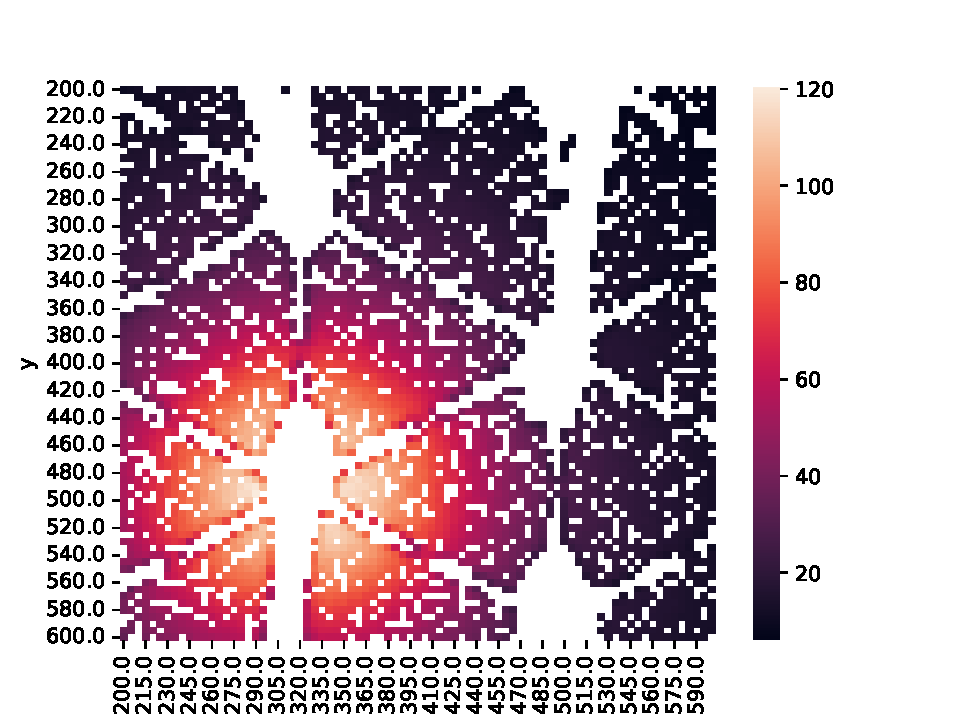
\includegraphics[scale=0.38]{images/pmax[5]_heatmap.pdf}}
\caption{Mean pmax[5] values grouping by (x, y) the development set}
\label{fig:pmax[5]_heatmap}
\end{figure}
\begin{figure}[htbp]
\centerline{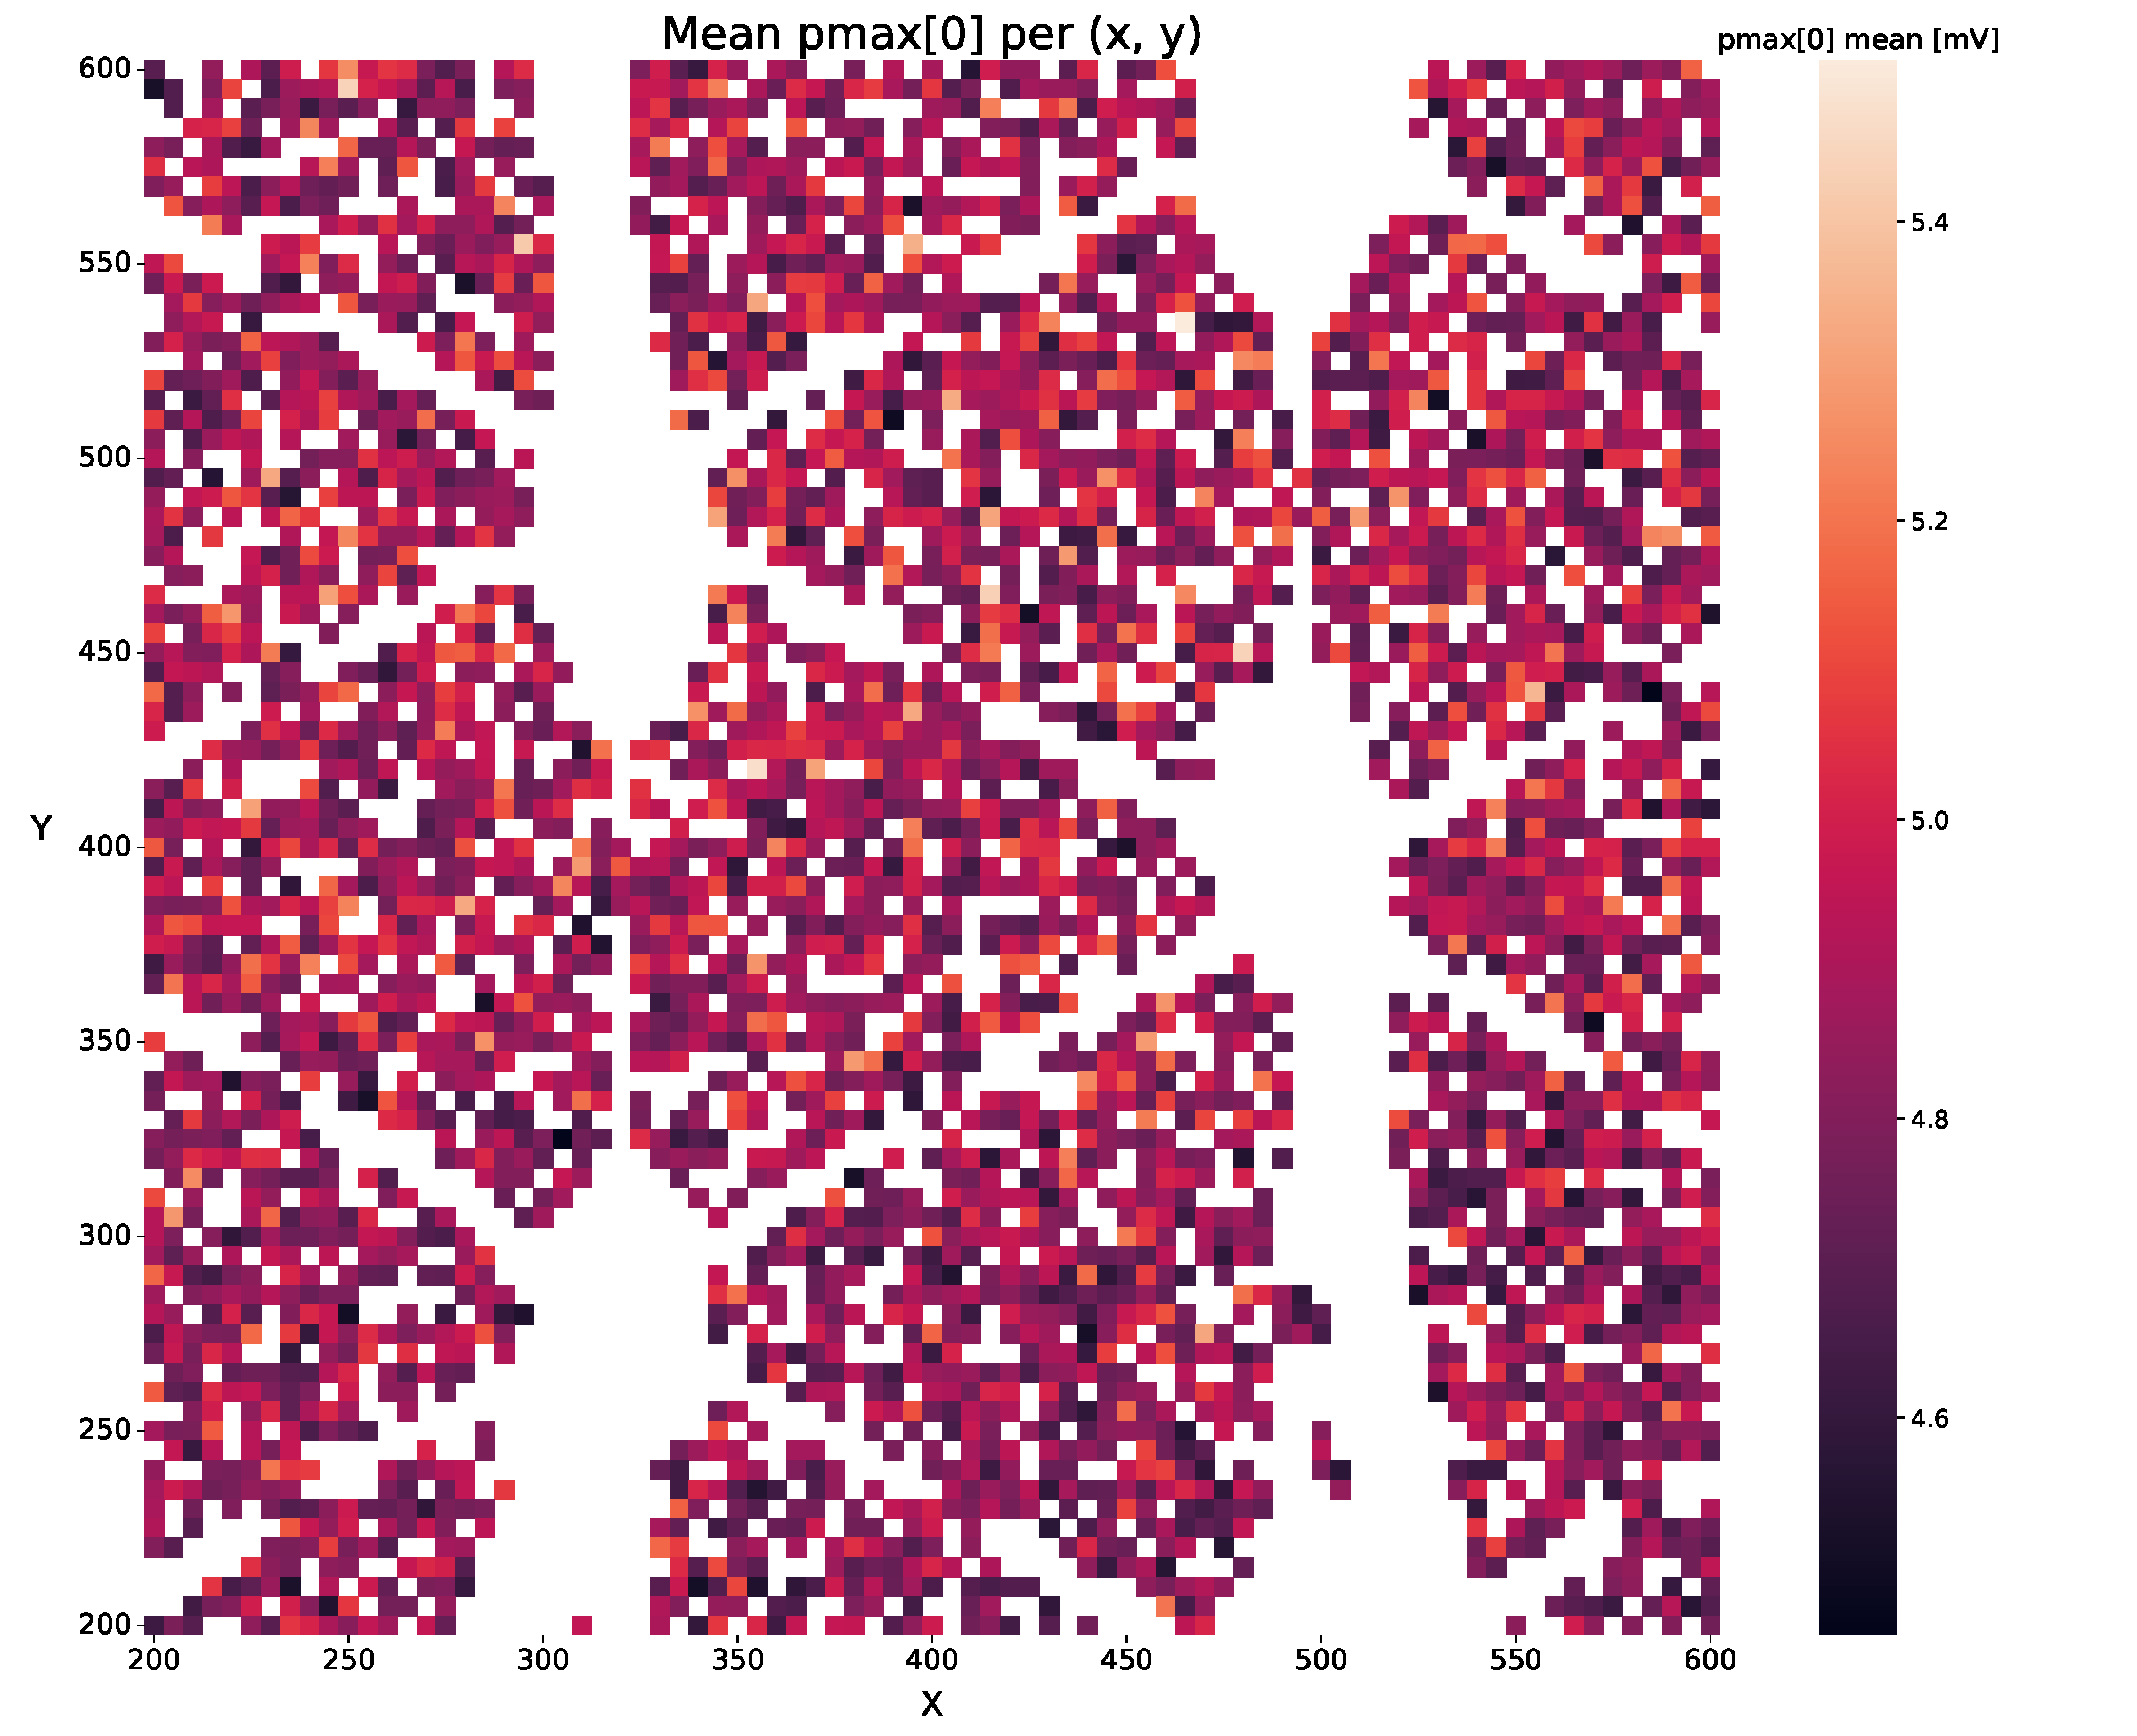
\includegraphics[scale=0.38]{images/pmax[0]_heatmap.pdf}}
\caption{Mean pmax[0] values grouping by (x, y) the development set}
\label{fig:pmax[0]_heatmap}
\end{figure}
A first observation is that for every $(x, y)$ present in the records, there are 100 events. The x and y values present are all the integers in the range $(200, 600)$ with step 5. Furthermore, not all the possible $(x, y)$ combinations are present as reported in Figure 
\ref{fig:pmax[5]_heatmap}. In particular, the positions of the pads can be identified by the complete absence of events. Only the shape of a few of them is complete because the positions collected are only of the central zone of the sensor. This is because when a particle hits the sensors, it does not pass through it and the event is not valid. \\%TODO: add a citation to a paper)

Figure \ref{fig:pmax[5]_heatmap} represents the mean pmax aggregating by $(x, y)$. Comparing the heat maps of the average pmax of different signals was useful for discerning the noise. An example is the difference between the figures \ref{fig:pmax[5]_heatmap} and \ref{fig:pmax[0]_heatmap}. The latter is clearly noise. \\
%(put the Figures of pmax[5] and pmax[0])
The same heat maps were used to identify the pad corresponding to each signal. The mean value of a specific pmax for a given $(x, y)$ is high only if the passing position of the particle is close to the pad. For instance, the pad corresponding to signal 5 is the one surrounded by cells encoded with brighter colors in Figure \ref{fig:pmax[5]_heatmap}.
The pad and the corresponding signal number are represented in Figure \ref{fig:rsd}.\\

\begin{figure}[htbp]
\centerline{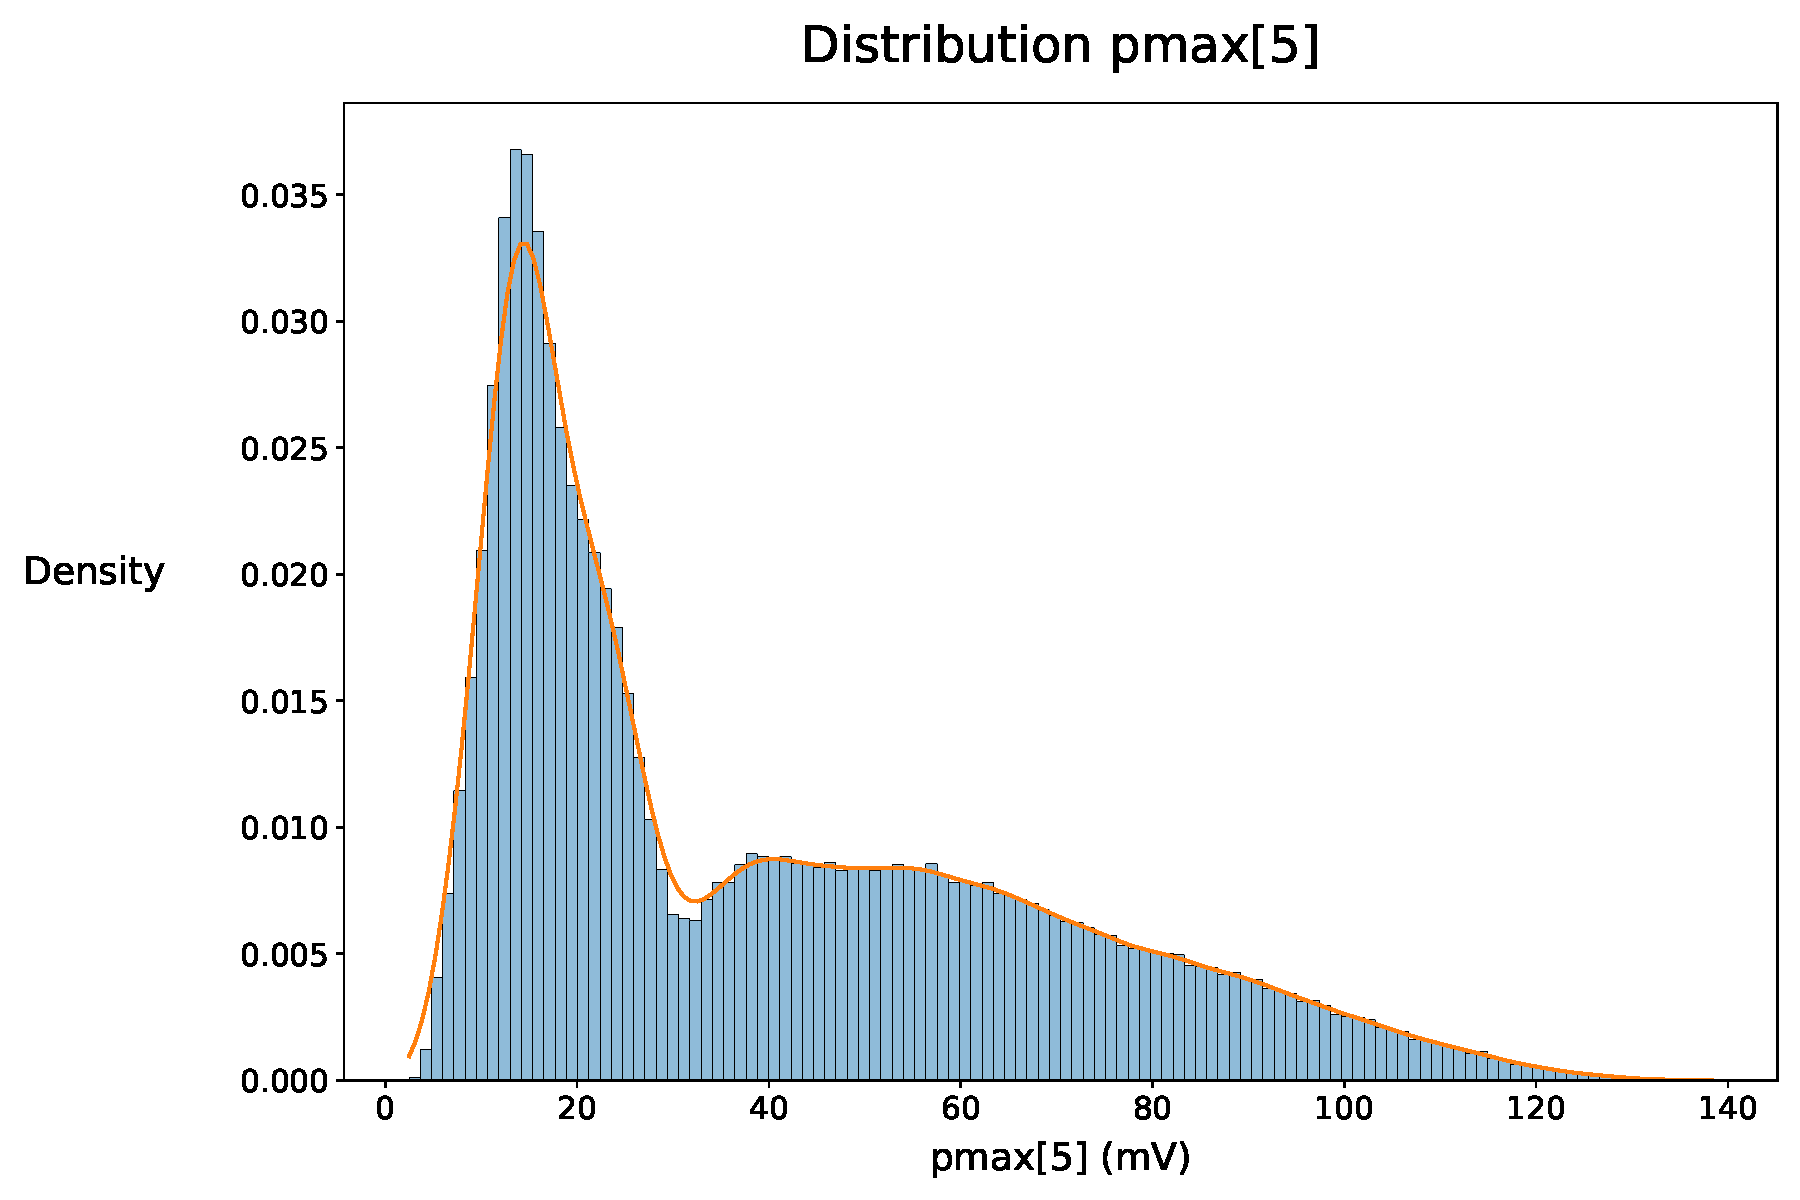
\includegraphics[scale=0.30]{images/pmax[5]_distr.pdf}}
\caption{Distribution of the pmax[5] values in the development set}
\label{fig:pmax[5]_distr}
\end{figure}
The difference between the noise and the signal can be also observed in the distributions of the values. A typical pmax probability function of a pad is represented in Figure \ref{fig:pmax[5]_distr}. The noise signals have completely different shapes and range of values. Most of the values have a low magnitude. This occurs because most of the time the pad is distant from the passing position.\\

The same analyses were performed on the other types presented in the listing \ref{lst:typeFeature}. Similar results were obtained for negpmax, area, and tmax. This confirmed that the features that share the same trailing "[n]" derive from the same signal. The tmax fields give less clear visualizations than the other three. On the other hand, the heat maps of the rms values do not present any visual pattern and the values are in the order of a few $mV$. The reason is that only a small portion of the signal can be characterized by peaks. Most of the time, the signal has a small magnitude of random noise. As a consequence, the latter part prevails in the computation of the rms.\\

%\begin{figure}[htbp]
%\centerline{\includegraphics[scale=0.35]%{images/negpmax_boxplot.pdf}}
%\caption{Negpmax boxplots}
%\label{fig:negpmax_boxplots}
%\end{figure}
Another consideration that can be made is on the distributions of negpmax. Its density functions have an unusual number of outliers compared to the other features. 

\section{Proposed approach}
\subsection{Preprocessing}

\begin{figure}[htbp]
\centerline{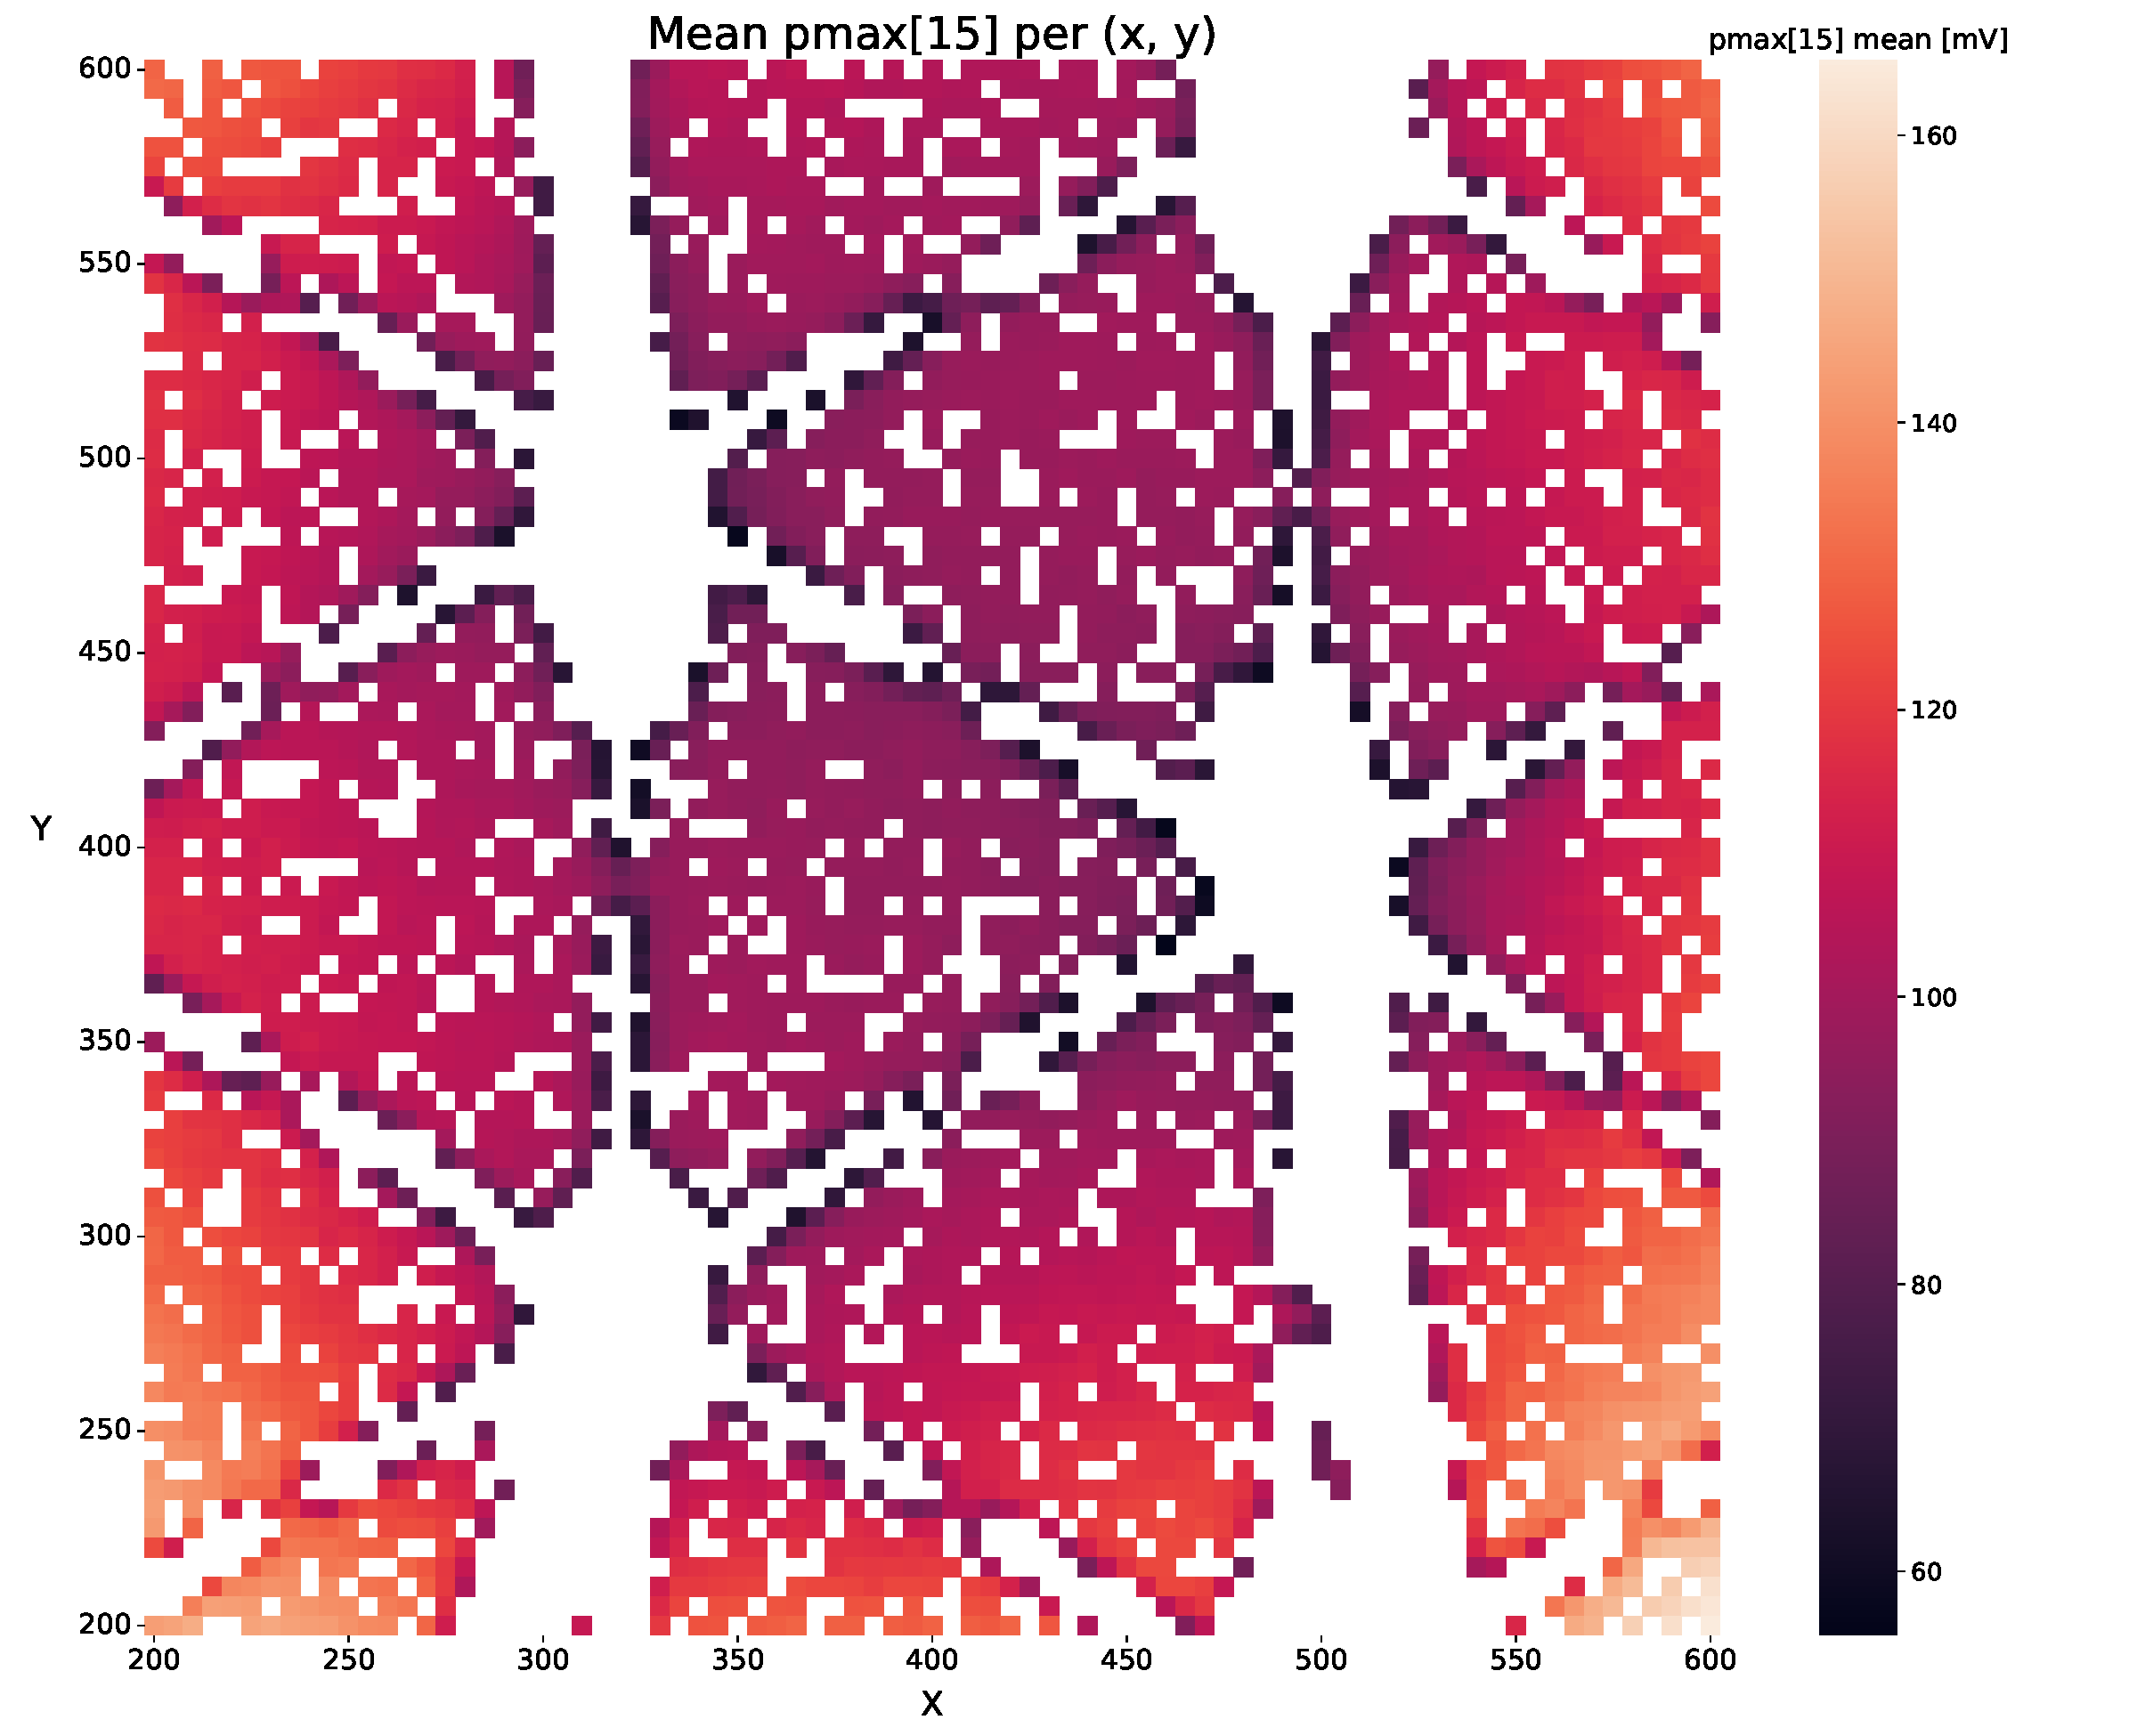
\includegraphics[scale=0.38]{images/pmax[15]_heatmap.pdf}}
\caption{Mean pmax[15] values grouping by (x, y) the development set}
\label{fig:pmax[15]_heatmap}
\end{figure}
We have seen from a visual perspective, which are the features that contain most of the information. These intuitive considerations were confirmed by an analysis of the importances obtained by a Random Forest regressor with default parameters. Only the pmax, negpmax, and the area of the signal derived from the pads were significantly used by the algorithm.\\ 
An interesting exception is the signal 15. Even if it should be only random noise, the $pmax[15]$ is taken into consideration. Observing Figure \ref{fig:pmax[15]_heatmap}, we see that the values are on average higher on the borders of the sensor and lower near the metal of the pads. Therefore, it contains useful information that can be used by the models. \\
For these reasons, we kept only pmax, negpmax, and the area of the signal corresponding to a pad and the feature $pmax[15]$.\\


In Section \ref{sec:problemOverview}, we have observed that only the columns of type negpmax contain many outliers. The magnitude of them is very different from the rest of the values. The same is not valid for the rest of the features. \\
We have also discussed that the absolute values are higher when the passing position is close to the sensor. Due to the broad range of x and y, often this does not happen. \\ 
To avoid the removal of useful data, we used the following procedure: we detected and saved the minimum negpmax for each row, and then we analyzed it using the Tukey's Fences method for outlier detection with coefficient k equal to 3. \\
The first step takes the measurements of the nearest pad for each event. In this way, we detected and removed the rows that contained negpmax values extremely different even for the closest pad.
 
\subsection{Model selection}
We have tested the following models:
\begin{itemize}
    \item Random forest(RT): it is an ensemble machine learning technique used for classification and regression. During the training phase, several decision trees are created on different random datasets, sampled with replacement from the original data. For a regression problem, the output of the random forest is the mean of the predictions of the single decision trees. Every split is learned during training considering a criterion, e.g. mean squared error, and possibly on a random subset of the features 
\cite{randomForest}] \cite{extraTree}.\\
The usage of multiple decision trees leads to a model more robust to noise \cite{randomForest}. The performance and the training times depend on the number of decision trees. The improvement provided by an increase in the number of decision trees is significant up to a certain number \cite{limitNumTrees}.\\
Even if the model is not interpretable as a decision tree, the overall importance of the features can still be obtained.
\item Extra-trees regressor(ET): it is an ensemble machine learning technique. There are only two main differences with the random forest method. The first is that every decision tree is built using the whole learning sample. The second is that the split is randomly selected from a uniform distribution inside the candidate feature's empirical range. Then among all the random splits, the best one is chosen and used to grow the tree. \\
The computational efficiency of the algorithm is an important advantage of this model \cite{extraTree}.
\item Voting regressor: it is an ensemble machine learning technique. It is based on the simple idea of using the average of different regression models. In this way, the advantages of multiple models can be combined. In this case, we used the mean of the random forest and the extra tree regressors. %TODO: cite a paper and change the name, I don't think that voting regressor is the official one
\end{itemize}
\subsection{Hyperparameters tuning}
The tuning was performed on the hyperparameters of the RT and the ET. As a consequence, the voting regressor used the best performing configurations of the other two models. \\
The RT and the ET algorithms share all the parameters we considered for the tuning, the parameters and their value are in table \ref{tab:tabHP}
\begin{table}
    \centering
    \caption{Hyperparameters considered}
    \label{tab:tabHP}
    \begin{tabular}{|c|c|c|}
        \hline
        \textbf{Model} & \textbf{Prameters} & \textbf{Values} \\
        \hline
        &criterion&Row 1\\
        Random Forest&max\_depth&Row 2\\
        &max\_features&Row 3\\
        \hline
        &criterion&Row 1\\
        Extra tree&max\_depth&Row 2\\
        &max\_features&Row 3\\
        \hline
    \end{tabular}
\end{table}
- the number of estimators $n\_estimators$
- the number of features considered at each split $max\_features$
- the maximum depth of each decision tree $max\_depth$
- the splitting criterion $criterion$

For the number of trees, the range $[64, 128]$ is suggested in many datasets\cite{limitNumTrees}. Over a certain threshold, increasing it does not improve significantly the performances, while extending considerably the computational time. \\
Also for this problem, it is not worth using over 128 estimators. \\
For this reason, we tested values of n\_estimators near 100. \\

The maximum depth obtained by the RT and the ET with default parameters is respectively 38 and 41. We tested the configurations with max\_depth:None\footnote{It does not impose any limits to the maximum depth of the trees}, 60\%, and 80\% of the previous values. 

We divided the development dataset 80/20. On the 80\%, we performed a cross validation using 4 folds. The metric used was the average Euclidean distance (\ref{eq:EuclideanDist}).\\
The 20\% was used to test the best performing models, before using all the labeled data to build the final regressors.
\section{Results}

%The feature selection process brought an important improvement to our solution, after the removal of the features that we decided to discard during the features analysis,
%our solution went from 5.039 to valore.
%5.039 Soluzione online base
%Distance on local test combined : 4.677499770610218
%Distance on local test randomF : 4.6320736739355395
%Distance on local test ET : 5.03086466714152
%Adding then the maximum pmax and the normalized pmax for each event improves our solution locally and on the online score board, the results we obtain

The tuning showed that for RF and ET the best configuration of hyper-parameters is very similar, the only difference was in "max features", 1.0 for ET and "sqrt" for RF.
The best configuration for RF was:

\begin{itemize}
    \item n\_estimators: 100
    \item criterion: "squared\_error"
    \item max\_features: "sqrt"
    \item max\_depth:None
\end{itemize}

The best configuration for ET was:
\begin{itemize}
    \item n\_estimators: 100
    \item criterion: "squared\_error"
    \item max\_features: 1.0
    \item max\_depth:None
\end{itemize}
In the end each step done from the pre-processing to the tuning improved the value of our solution, that in the end was 4.637 on the pubblic scoreboard, while the the score that is obtained only training the regressors on the original development set is 5.039.
During the discussion every time we refer to local tests, they are test done splitting the development set and doing the training on 80\% of it and the testing on the 20\% of it. Instead to label the evaluation set and upload our submission on the public scoreboard we trained the regressor on 100\% of the developement set
One thing that we observed was that, for local test, the distance obtained at the end of the process, for the RT was 4.261, for ET was 3.907 and 3.990 for VR, but when we do our tests online we can see that the best score is obtained with V. We may assume that this happens because VR take the advantages of the regressors, that are very similar in this case, and merge them, in this way it works better when in the evaluation set it finds data that were not in the training set.



We also defined a naive regressor to compare our solution with it. The naive solution just predicts the average between xmax and xmin, where xmax is the maximum value of x in the development dataset and xmin is the minimum, and it does the same reasoning for the y.
The solution of the naive one was valore.

Finally we can notice that our proposed solution it is considerably better than the baseline that we can find in the scoreboard, the difference between the two is 1.992.

If we compare our result with the ones obtained by other grups on the scoreaboard, we can see that we are on the first third of the table, for sure there is room for improvement considering that the solutions in the first positions are significantly superior.

\section{Discussion}
From the results we obtained we can see that the predictions done with the VR are closer to the solution than the ones we obtained using the algorithms separetly, this is what we expected from the voting regressor, that with similar algorithms is supposed to exploit the advantages of them and obtain better results.
We also wanted to underline that it is possible to notice that prediction error is bigger near the pads of the sensors, in those positions we can see that the error is bigger if compared to others not so close to the pads.
To seek a solution that improves the proposed one it is possibile to expand the grid search testing more configuration for the attributes on which we focused, it could be also interesting to add more attributes to the grid search. 
Different and improved results could be found trying various technique, methods that exploits other Machine Learning regressor that we did not explore.
Also additional domain knowledge, like pyhisical consideration on the particle or on the sensonr, could help during the feature extraction.
% used in veichle perception and localisation, it is a different field of study but it is still a spatial resolution problem, paper [4] shows Different approaches that have been used in this field in the past years
%TODO: I would stay general and say that physical considerations about the particles could help improve the feature extraction
In the end, taking as reference the baseline, we are satisfied by the solution obtained using our approach.


\bibliography{bibliography}
\bibliographystyle{ieeetr}

\end{document}